\lab{Linear Transformations}{Linear Transformations}
\objective{One of the most important questions in scientific computing is ``How long will a computer take to execute this algorithm?'' In this lab we explore why NumPy is a good option for performing numerical linear algebra.
Linear transformations are the most basic and essential operations in vector space theory; we visually explore how linear transformations alter points in $\mathbb{R}^2$.
}
% \objective{Apply affine transformations to a set of vectors in $\mathbb{R}^2$.}
% \objective{Introduce the temporal and spatial complexity and explore SciPy's methods for working with sparse matrices.}

\section*{Matrix Operations} % ================================================

\subsection*{Timing Code} % ---------------------------------------------------

The \li{time} module in the standard library include functions for dealing with time.
The module's \li{time()} function measures the number of seconds from a fixed starting point, called ``the Epoch'' (January 1, 1970 for Unix machines).

\begin{lstlisting}
>>> import time
>>> time.time()
1466609325.819298
\end{lstlisting}

The \li{time()} function\footnote{The \li{clock()} function is similar to \li{time()}, but it records more precision on Windows machines.} is useful for measuring how long it takes for code to run: record the time just before and just after the code in question, then subtract the first measurement from the second to get the number of seconds that have passed.

\begin{lstlisting}
>>> def time_for_loop(iters):
...     """Time how long it takes to go through 'iters' iterations of nothing."""
...     start = time.time()         # Clock the starting time.
...     for _ in range(int(iters)):
...         pass
...     end = time.time()           # Clock the ending time.
...     return end - start          # Report the difference.
...
>>> time_for_loop(1e5)              # 1e5 = 100000.
0.007936954498291016
>>> time_for_loop(1e7)              # 1e7 = 10000000.
0.8008430004119873
\end{lstlisting}

The standard library's \li{timeit} module is built specifically to time code and has more sophisticated tools than the \li{time} module.
The \li{timeit()} function accepts a function handle (the name of the function to run) and the number of times to run it.
Additionally, in IPython the quick command \li{\%timeit} uses \li{timeit.timeit()} to quickly time a single line of code.

\begin{lstlisting}
In [1]: import timeit
In [2]: def for_loop():
   ...:     """Go through 1e7 iterations of nothing."""
   ...:     for _ in range(int(1e7)):
   ...:         pass

In [3]: timeit.timeit(for_loop, number=5) / 5.
Out[3]: 0.8081045627593995

In [4]: %timeit for_loop()
1 loop, best of 3: 801 ms per loop
\end{lstlisting}

\subsection*{Timing an Algorithm} % -------------------------------------------

Most algorithms have at least one input that dictates the size of the problem to be solved.
For example, the following functions take in a single integer $n$ and produce a random vector of length $n$ as a list or a random $n\times n$ matrix as a list of lists:

\begin{lstlisting}
from random import random

def random_vector(n):
    """Generate a random vector of length n as a list."""
    return [random() for i in xrange(n)]

def random_matrix(n):
    """Generate a random nxn matrix as a list of lists."""
    return [[random() for j in xrange(n)] for i in xrange(n)]
\end{lstlisting}

Executing \li{random_vector(n)} calls \li{random()} $n$ times, so doubling $n$ should about double the amount of time \li{random_vector(n)} takes to execute.
By contrast, executing \li{random_matrix(n)} calls \li{random()} $n^2$ times ($n$ times per row with $n$ rows).
Therefore doubling $n$ will likely more than double the amount of time \li{random_matrix(n)} takes to execute, especially if $n$ is large.

To visualize this phenomenon, we time \li{random_matrix()} for $n = 2^1,\ 2^2,\ \ldots,\ 2^{12}$ and plot $n$ against the execution time.
The result is displayed below on the left.% in Figure \ref{fig:matrix_time_result1}.

\begin{lstlisting}
>>> from matplotlib import pyplot as plt
>>> domain = 2**np.arange(1,13)
>>> times = []
>>> for n in domain:
...     start = time.time()
...     random_matrix(n)
...     times.append(time.time() - start)
...
>>> plt.plot(domain, times, 'g.-', linewidth=2, markersize=15)
>>> plt.xlabel("n", fontsize=14)
>>> plt.ylabel("Seconds", fontsize=14)
>>> plt.show()
\end{lstlisting}

\begin{figure}[H] % Generated with timing_demo() in plots.py.
\captionsetup[subfigure]{justification=centering}
\centering
\begin{subfigure}{.5\textwidth}
    \centering
    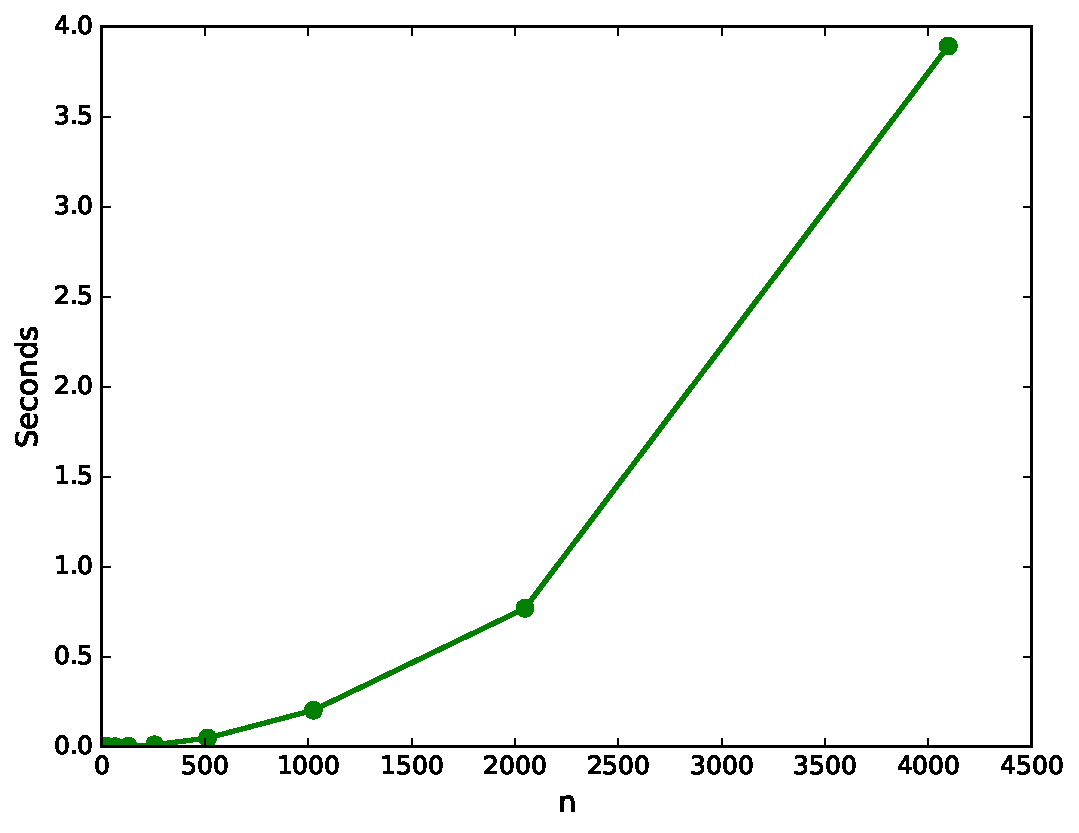
\includegraphics[width=\linewidth]{time_random_matrix1.pdf}
    % \label{fig:matrix_time_result1}
\end{subfigure}%
\begin{subfigure}{.5\textwidth}
    \centering
    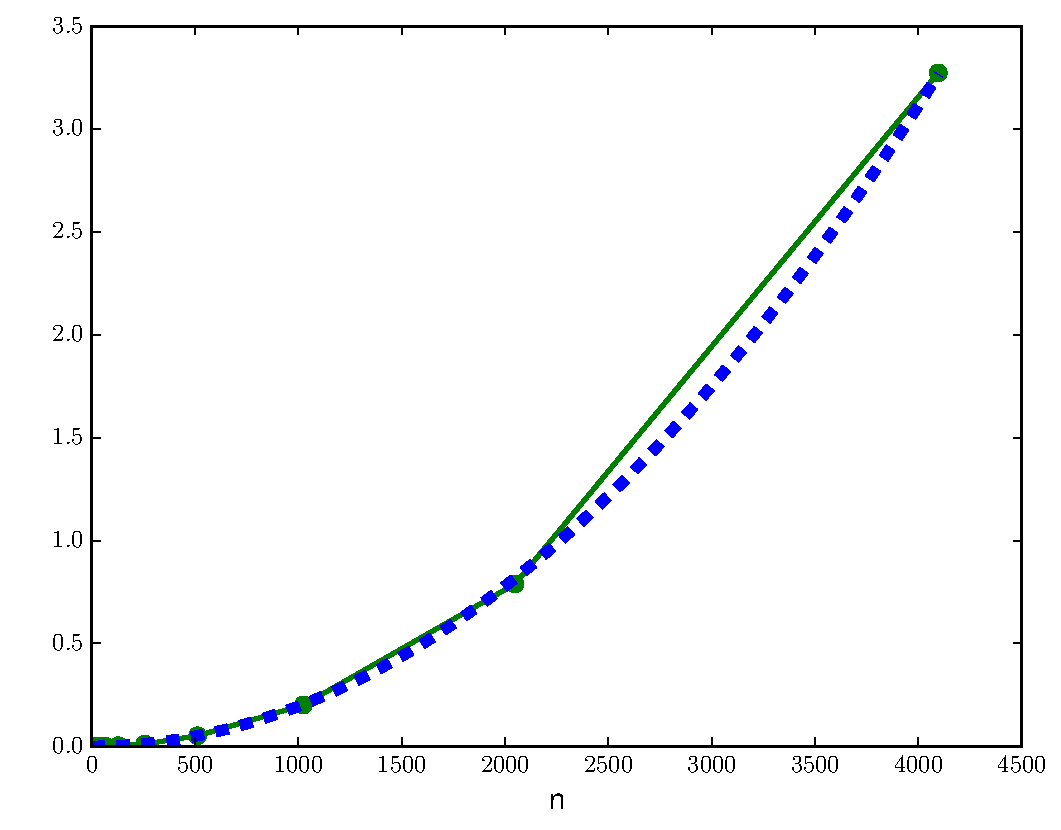
\includegraphics[width=\linewidth]{time_random_matrix2.pdf}
\end{subfigure}
\end{figure}

The figure on the left shows that the execution time for \li{random_matrix(n)} increases quadratically in $n$.
In fact, the blue dotted line in the figure on the right is the parabola $y = an^2$, which fits nicely over the timed observations. Here $a$ is a small constant, but it is much less significant than the exponent on the $n$---we can leave it off altogether and write \li{random_matrix(n)} $\sim n^2$.%\footnote{In precise mathematical terms, we might write \li{random_matrix(n)} $\in O(n^2)$. See Volume II for more details on Big-O notation.}

% TODO: More explanation here? Reference to Vol II?

\begin{problem} % Time Matrix-Vector and Matrix-Matrix Multiplication.
Let $A$ be an $m \times n$ matrix with entries $a_{ij}$, $\x$ be an $n \times 1$ vector with entries $x_k$, and $B$ be an $n \times p$ matrix with entries $b_{ij}$.
%
\begin{align*}
A = \left[\begin{array}{cccc}
a_{11} & a_{12} & \cdots & a_{1n} \\
a_{21} & a_{22} & \cdots & a_{2n} \\
\vdots & \vdots & \ddots & \vdots \\
a_{m1} & a_{m2} & \cdots & a_{mn}
\end{array}\right]
&&
\x = \left[\begin{array}{c}
x_1 \\ x_2 \\ \vdots \\ x_n
\end{array}\right]
&&
B = \left[\begin{array}{cccc}
b_{11} & b_{12} & \cdots & b_{1p} \\
b_{21} & b_{22} & \cdots & b_{2p} \\
\vdots & \vdots & \ddots & \vdots \\
b_{n1} & b_{n2} & \cdots & b_{np}
\end{array}\right]
\end{align*}

The matrix-vector product $A\x = \y$ is a new $m \times 1$ vector and the matrix-matrix product $AB = C$ is a new $m \times p$ matrix.
The entries $y_i$ of $\y$ and $c_{ij}$ of $C$ are determined by the following formulas:
%
\begin{align*}
y_i = \sum_{k=1}^n a_{ik}x_k%,\qquad i = 1,\ 2,\ \ldots,\ m.
&&
c_{ij} = \sum_{k=1}^n a_{ik}b_{kj}%,\quad i = 1,\, 2,\, \ldots,\ m, \quad j = 1,\, 2\, \ldots,\ l.
\end{align*}

Below, we implement these multiplication formulas without using NumPy.

\begin{lstlisting}
def matrix_vector_product(A, x):
    """Compute the matrix-vector product Ax (as a list)."""
    m, n = len(A), len(x)
    return [sum([A[i][k] * x[k] for k in range(n)]) for i in range(m)]

def matrix_matrix_product(A, B):
    """Compute the matrix-matrix product AB (as a list of lists)."""
    m, n, p = len(A), len(B), len(B[0])
    return [[sum([A[i][k] * B[k][j] for k in range(n)])
                                    for j in range(p) ]
                                    for i in range(m) ]
\end{lstlisting}

Use \li{time.time()}, \li{timeit.timeit()}, or \li{\%timeit} to time each of these functions with increasingly large inputs.
Generate the inputs $A$, $\x$, and $B$ with \li{random_matrix()} and \li{random_vector()} (so each input will be $n \times n$ or $n \times 1$).
Only time the multiplication functions, not the generating functions.

Report your findings in a single figure with two subplots: one with matrix-vector times, and one with matrix-matrix times.
Choose a domain for $n$ so that your figure accurately describes the growth, but avoid values of $n$ that lead to execution times of more than 1 minute.
Your figure should resemble the following plots.

\begin{figure}[H] % Generated with prob1_solution() in plots.py.
\captionsetup[subfigure]{justification=centering}
\centering
\begin{subfigure}{.5\textwidth}
    \centering
    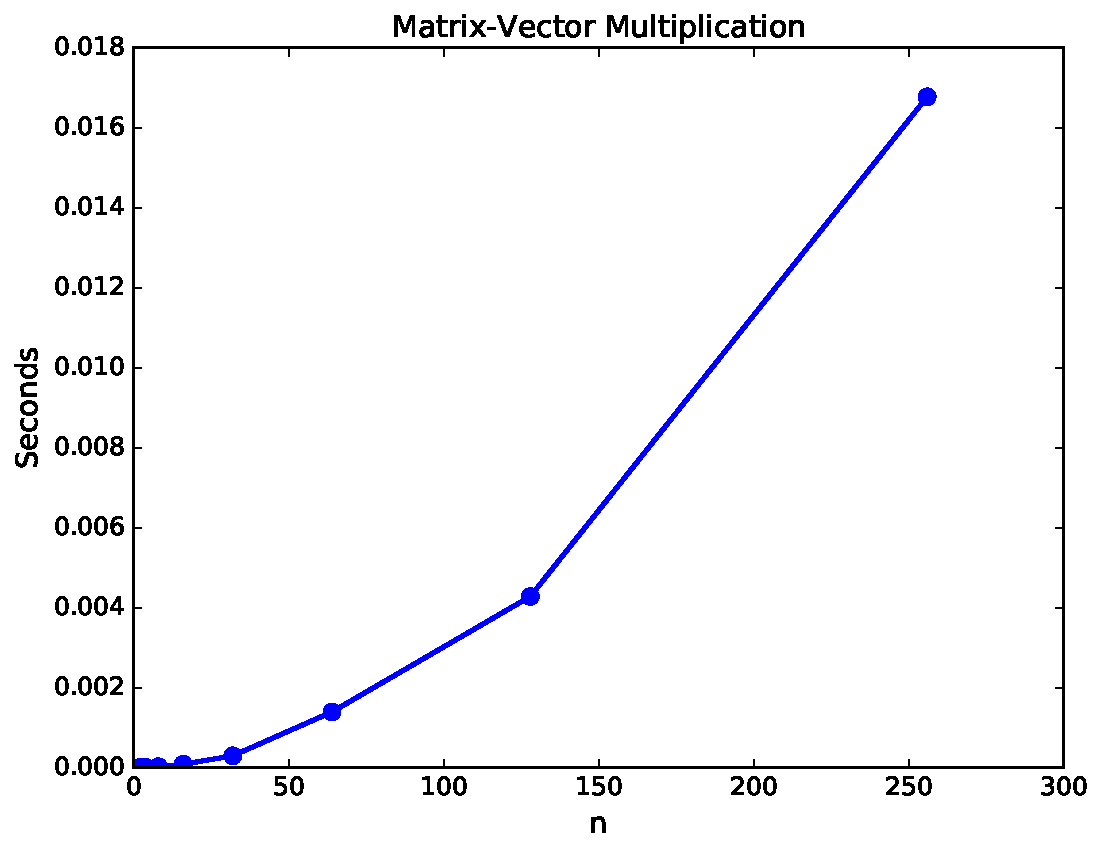
\includegraphics[width=\linewidth]{matrixVectorMultiplication.pdf}
\end{subfigure}%
\begin{subfigure}{.474\textwidth}
    \centering
    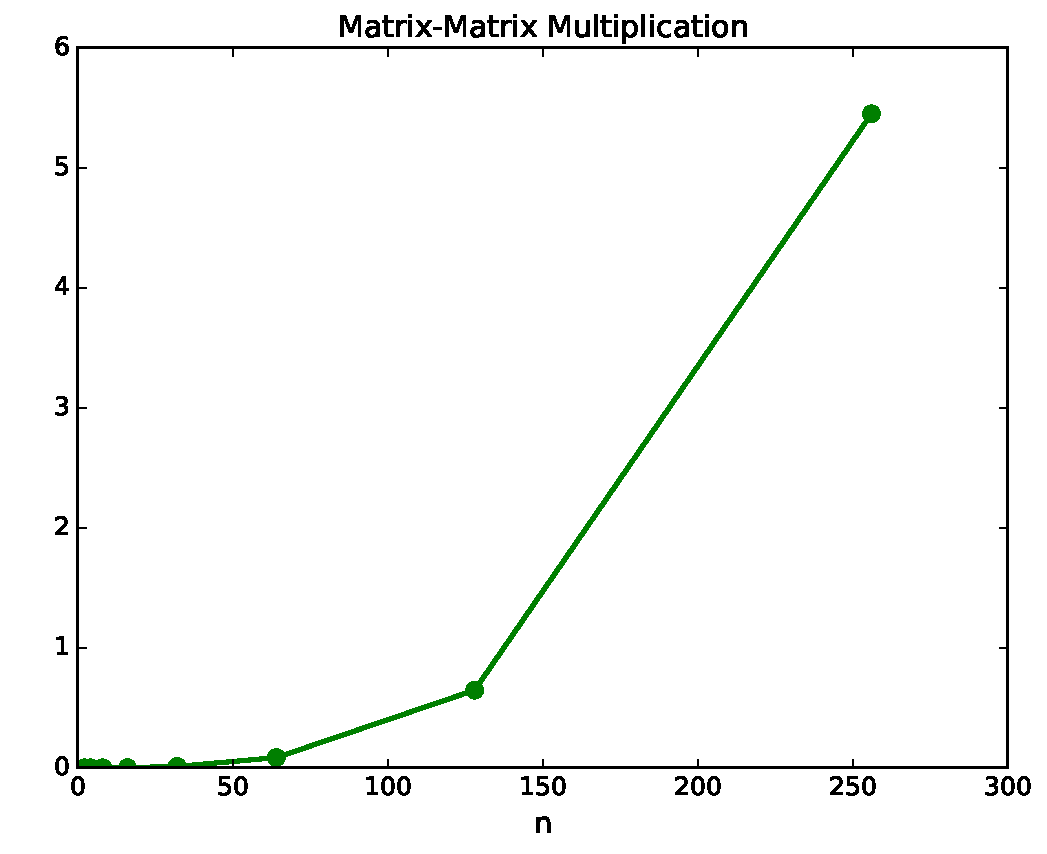
\includegraphics[width=\linewidth]{matrixMatrixMultiplication.pdf}
\end{subfigure}
\end{figure}

\label{prob:matrix-multiplication-timing}
\end{problem}

\subsection*{Logarithmic Plots} % ---------------------------------------------

The two plots from Problem \ref{prob:matrix-multiplication-timing} look similar, but the actual execution times differ greatly.
To adequately compare the two, we need to view the results differently.

A \emph{logarithmic plot} uses a logarithmic scale---with values that increase exponentially, such as $10^1,\ 10^2,\ 10^3,\ \ldots$---on one or both of its axes.
The three kinds of log plots are listed below.

\begin{itemize}
\item \textbf{log-lin}: the $x$-axis uses a logarithmic scale but the $y$-axis uses a linear scale.\\
Use \li{plt.semilogx()} instead of \li{plt.plot()}.
\item \textbf{lin-log}: the $x$-axis is uses a linear scale but the $y$-axis uses a log scale.\\
Use \li{plt.semilogy()} instead of \li{plt.plot()}.
\item \textbf{log-log}: both the $x$ and $y$-axis use a logarithmic scale.\\
Use \li{plt.loglog()} instead of \li{plt.plot()}.
\end{itemize}

Since the domain $n = 2^1,\ 2^2,\ \ldots$ is a logarithmic scale and the execution times increase quadratically, we visualize the results of the previous problem with a log-log plot.
The default base for the logarithmic scales on logarithmic plots in Matplotlib is $10$.
To change the base to $2$ on each axis, specify the keyword arguments \li{basex=2} and \li{basey=2}.

Suppose the domain of $n$ values are stored in \li{domain} and the corresponding execution times for \li{matrix_vector_product()} and \li{matrix_matrix_product()} are stored in \li{vector_times} and \li{matrix_times}, respectively.
The following code produces Figure \ref{fig:loglogdemo}.

\begin{lstlisting}
>>> plt.subplot(121)        # Plot both curves on a lin-lin plot.
>>> plt.plot(domain, vector_times, 'b.-', lw=2, ms=15, label="Matrix-Vector")
>>> plt.plot(domain, matrix_times, 'g.-', lw=2, ms=15, label="Matrix-Matrix")
>>> plt.legend(loc="upper left")

>>> plot.subplot(122)       # Plot both curves on a base 2 log-log plot.
>>> plt.loglog(domain, vector_times, 'b.-', basex=2, basey=2, lw=2, ms=15)
>>> plt.loglog(domain, matrix_times, 'g.-', basex=2, basey=2, lw=2, ms=15)
>>> plt.show()
\end{lstlisting}

\begin{figure}[H] % Generated with loglog_demo() in plots.py.
\captionsetup[subfigure]{justification=centering}
\centering
\begin{subfigure}{.5\textwidth}
    \centering
    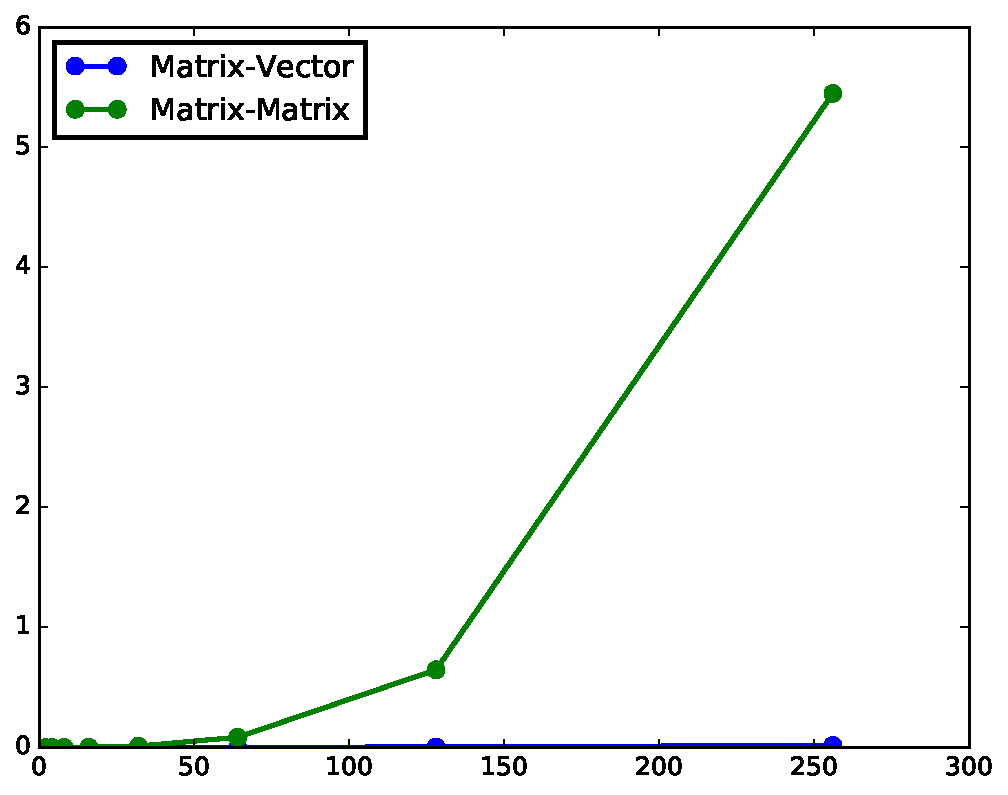
\includegraphics[width=\linewidth]{loglogDemoBad.pdf}
\end{subfigure}%
\begin{subfigure}{.5\textwidth}
    \centering
    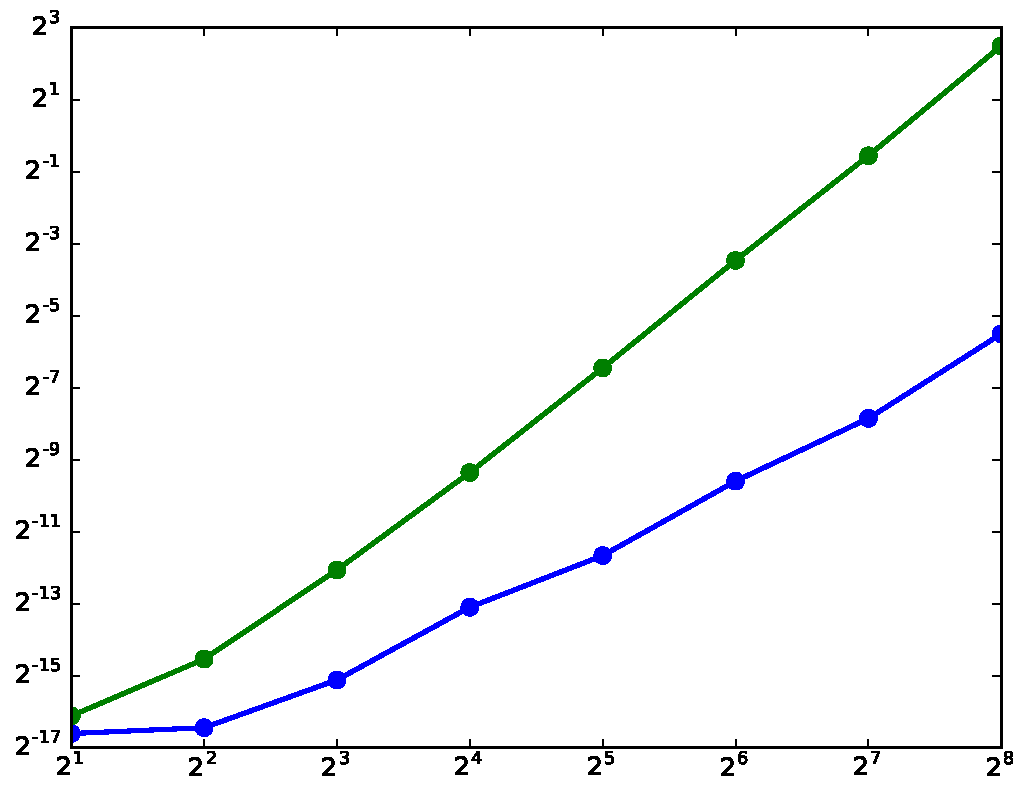
\includegraphics[width=\linewidth]{loglogDemoGood.pdf}
\end{subfigure}
\caption{ }
\label{fig:loglogdemo}
\end{figure}

Since the slope of the line for \li{matrix_matrix_product()} is noticeably greater than the slope of the \li{matrix_vector_product()} line, we conclude that matrix-matrix multiplication is an order of magnitude faster than matrix-matrix multiplication.
In fact, matrix-matrix multiplication (which uses 3 \li{for} loops) is $\sim n^3$, while matrix-vector multiplication (which only has 2 loops) is only $\sim n^2$.

\begin{problem} % Why NumPy ROCKS.
NumPy is optimized for fast computations.
Repeat the experiment of Problem \ref{prob:matrix-multiplication-timing}, timing the following operations:
%
\begin{itemize}
\item matrix-vector multiplication with \li{matrix_vector_product()}.
\item matrix-matrix multiplication with \li{matrix_matrix_product()}.
\item matrix-vector multiplication with \li{np.dot()}.
\item matrix-matrix multiplication with \li{np.dot()}.
\end{itemize}

Create a single figure with two subplots: one with all four sets of execution times on a regular linear scale, and one with all four sets of execution times on a log-log scale.
Compare your results to Figure \ref{fig:loglogdemo}.
\end{problem}

Apart from being syntactically convenient, element-wise NumPy operations are also significantly faster than element-wise list operations.
The coefficient for list of lists is way bigger than it is with NumPy arrays.
Iterating through loops is very expensive.
NumPy also uses loops, but it uses C loops instead of Python loops.

\begin{info} % Note about Caching.
The execution times for matrix multiplication with NumPy increase somewhat erratically.
NumPy operations are optimized for computer hardware.
Below, we plot execution times for vector-vector multiplication with NumPy.
The spikes in the plot indicate the times that the array no longer fits in the current level of memory
%
\begin{figure}[H]
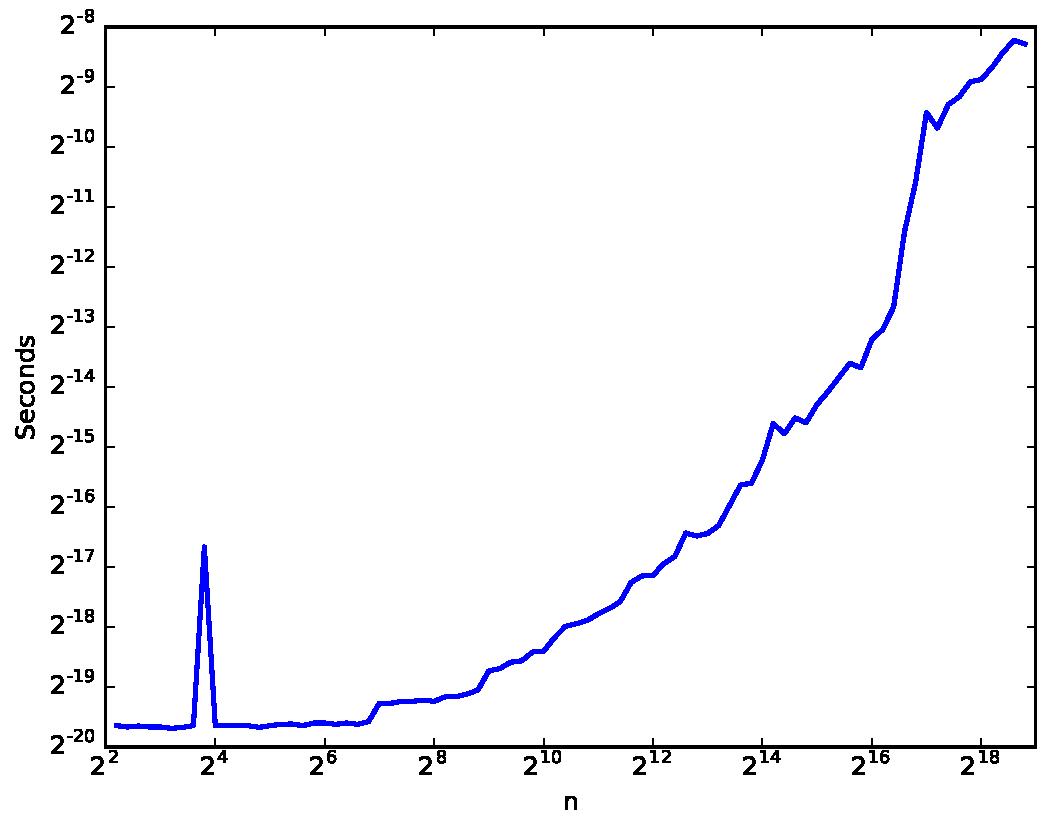
\includegraphics[width=.5\textwidth]{cachingDemo.pdf}
\end{figure}
\end{info}

\section*{Linear Transformations} % ===========================================

A \emph{linear transformation} is a mapping on a vector space that preserves addition and scalar multiplication.
More precisely, for an arbitrary vector space $V$, the mapping $L:V\rightarrow V$ is a linear transformation if and only if it satisfies the following conditions:
%
\begin{itemize}
\item $T(\x + \y) = T\x + T\y$ for any two vectors $\x,\ \y \in V$
\item $T(\alpha\x) = \alpha T\x$ for any vector $\x \in V$ and any scalar $\alpha \in \mathbb{F}$.
\end{itemize}

In $\mathbb{R}^n$, every linear transformation $L$ can be represented by an $n \times n$ matrix $A$.
To apply $L$ to a vector $\x \in \mathbb{R}^n$, left multiply by the matrix representation.


\subsection*{Dilations}
A \emph{dilation} of the vector space rescales the vectors.
Graphically, a dilation stretches or compresses the space.
A linear transformation is a dilation if and only if its matrix representation is diagonal, so in particular all Type II elementary matrices are dilations.
The matrix $\begin{pmatrix}1.25 & 0\\0 & .25 \end{pmatrix}$ corresponds to the dilation below.

\begin{figure}[H] % Generated with dilated_horse() in plots.py.
\captionsetup[subfigure]{justification=centering}
\centering
\begin{subfigure}{.5\textwidth}
    \centering
    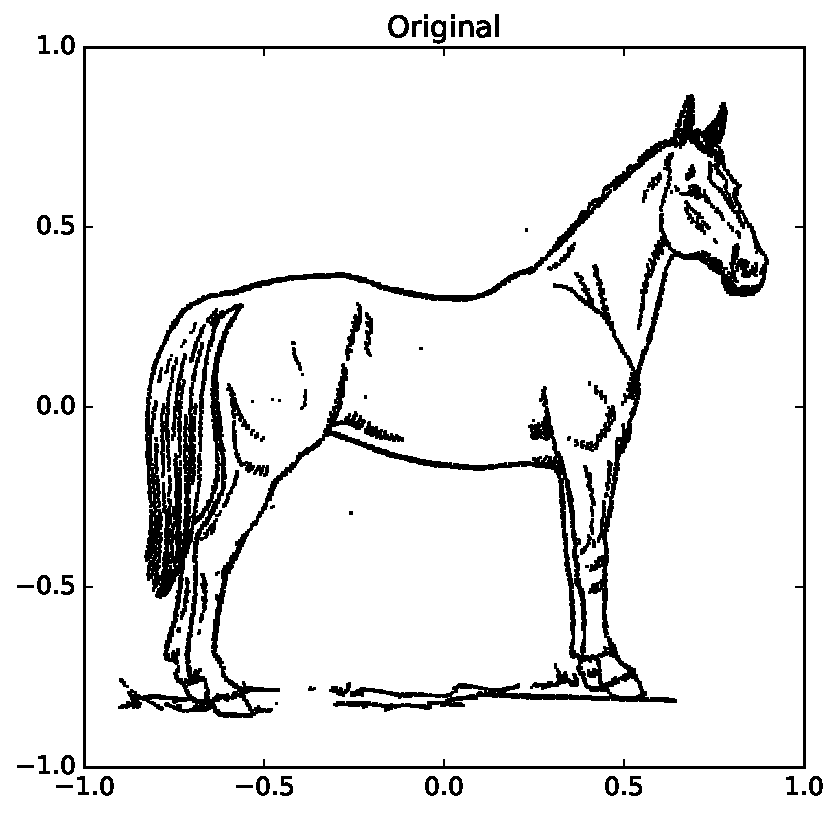
\includegraphics[width=\linewidth]{originalHorse.pdf}
\end{subfigure}%
\begin{subfigure}{.5\textwidth}
    \centering
    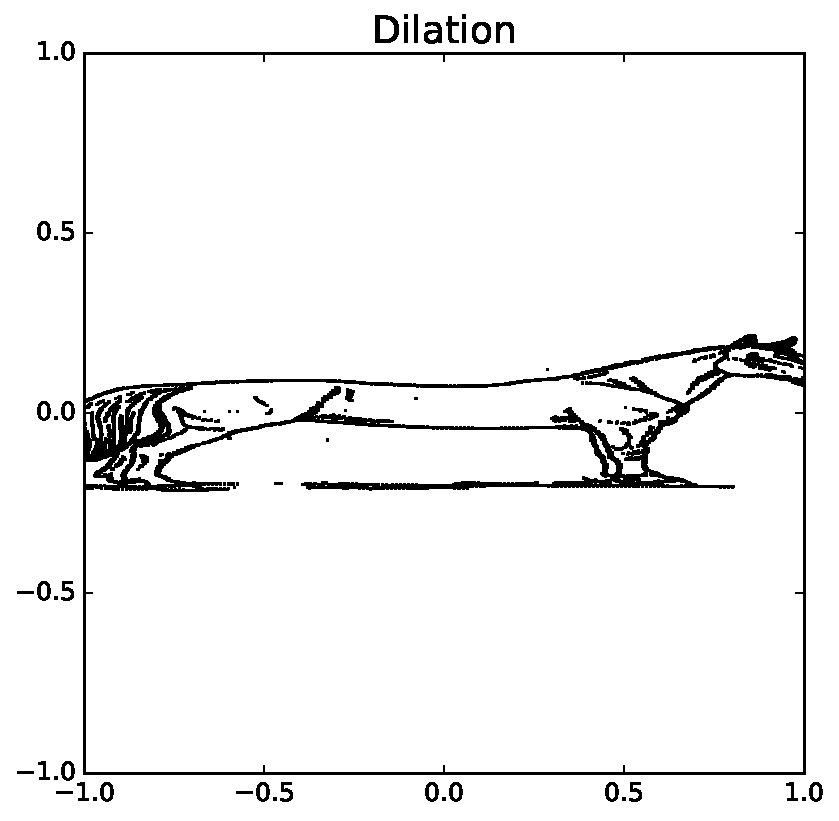
\includegraphics[width=\linewidth]{DilationHorse.pdf}
\end{subfigure}
\end{figure}

\begin{problem}
Write a function that accepts an array of points and an array giving the stretching factors in each direction.
Your function should return the dilated points.
\label{prob:dilation}
\end{problem}

\subsection*{Rotations} % -----------------------------------------------------

A second type of linear transformation is to rotate vectors around the origin.
A rotation of $\theta$ radians counterclockwise corresponds to the matrix $\begin{pmatrix}
\cos(\theta) & -\sin(\theta) \\
\sin(\theta) & \cos(\theta)
\end{pmatrix}.$
Rotating with $\theta = \pi/3$ produces the figure shown below.

\begin{figure}[H] % Generated with rotated_horse() in plots.py.
\captionsetup[subfigure]{justification=centering}
\centering
\begin{subfigure}{.5\textwidth}
    \centering
    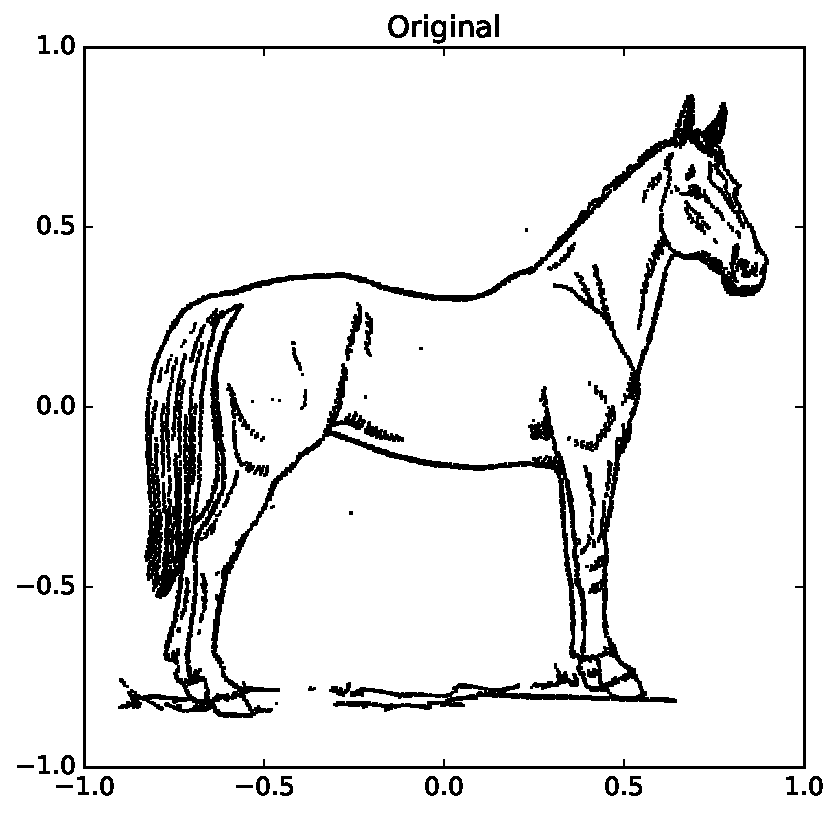
\includegraphics[width=\linewidth]{originalHorse.pdf}
\end{subfigure}%
\begin{subfigure}{.5\textwidth}
    \centering
    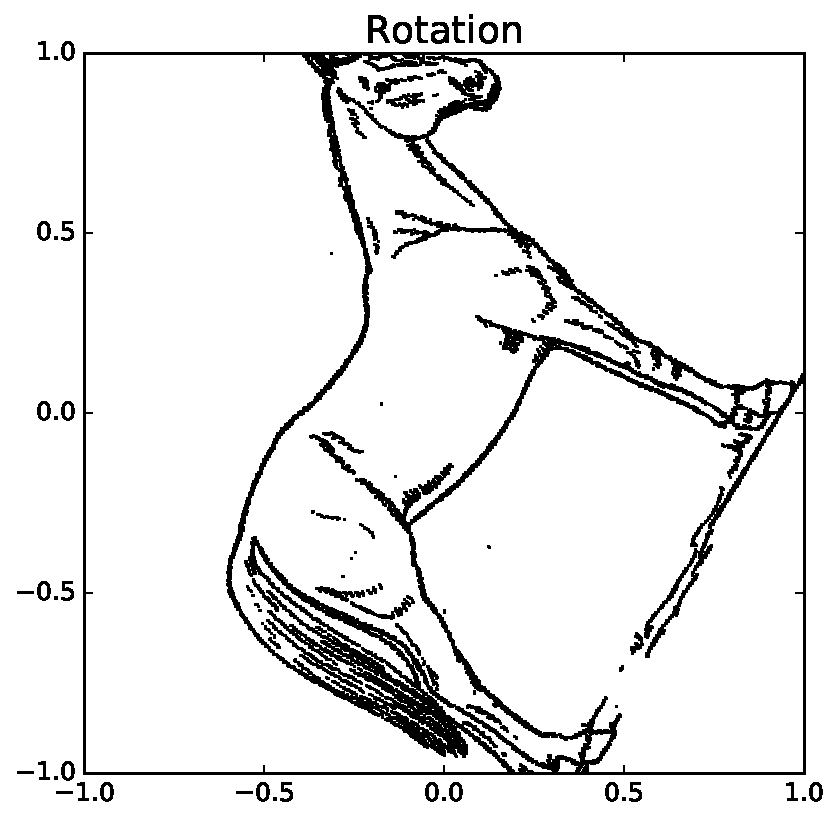
\includegraphics[width=\linewidth]{RotationHorse.pdf}
\end{subfigure}
\label{fig:rotate}
\end{figure}

\begin{problem}
Write a function that accepts an array of points and the angle of rotation (in radians).
Your function should return the rotated points.
\end{problem}

\subsection*{Shears} % --------------------------------------------------------

A third type of linear transformation is a \emph{shear}, which ``slants'' a set of vectors.
The corresponding matrix is a Type III elementary matrix.
A horizontal shear has the form $\begin{pmatrix}
1 & c \\
0 & 1
\end{pmatrix}$ and a vertical skew has the form $
 \begin{pmatrix}
1 & 0 \\
c & 1
\end{pmatrix}
$.
Horizontal skews fix the $y$-coordinate of a vector while vertical skews fix the $x$-coordinate.
The horizontal shear shown below corresponds to the matrix $\begin{pmatrix}
1 & .2 \\
0 & 1
\end{pmatrix}
$.

\begin{figure}[H] % Generated with dilated_horse() in plots.py.
\captionsetup[subfigure]{justification=centering}
\centering
\begin{subfigure}{.5\textwidth}
    \centering
    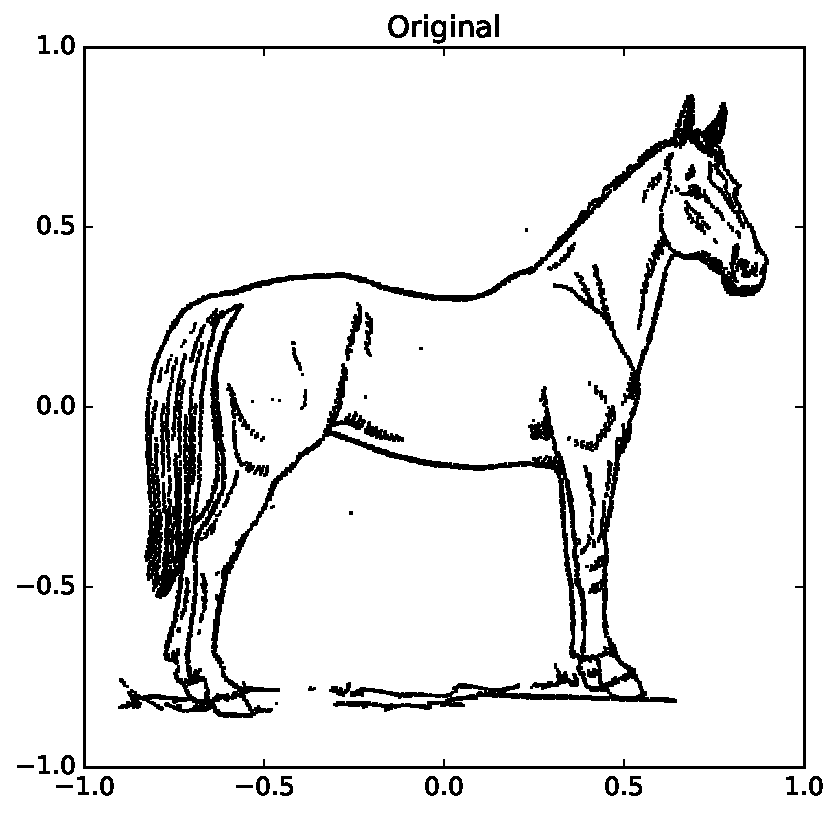
\includegraphics[width=\linewidth]{originalHorse.pdf}
\end{subfigure}%
\begin{subfigure}{.5\textwidth}
    \centering
    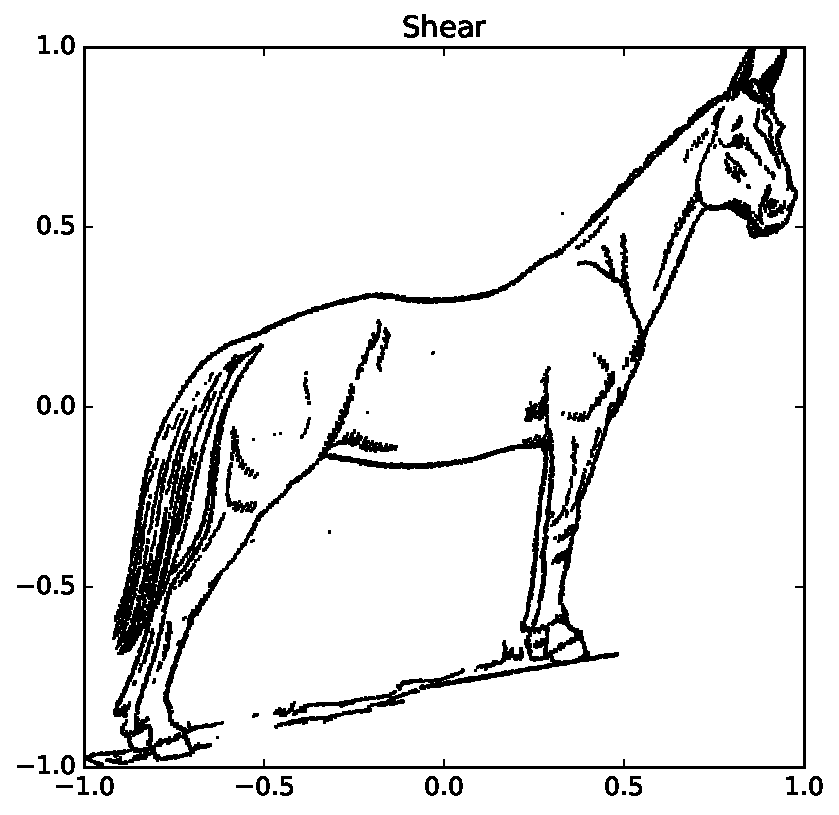
\includegraphics[width=\linewidth]{ShearHorse.pdf}
\end{subfigure}
\end{figure}


\begin{problem}
Write a function that accepts an array of points, a floating point argument that indicates the shearing amount, and an integer argument that indicates the direction of the shear (0 for horizontal, 1 for vertical).
Your function should return the sheared points.
\end{problem}

\subsection*{Reflections}% ----------------------------------------------------

A fourth type of linear transformation is reflections about a line, also called \emph{Householder transformations}.
Reflecting about a line spanned by $(l_1, l_2)$ corresponds to the matrix
\[
\frac{1}{l_1^2 + l_2^2}
\begin{pmatrix}
l_1^2 - l_2^2 & 2l_1l_2 \\
2l_1l_2 & l_2^2 - l_1^2
\end{pmatrix}.
\]

For example, the line $y=x$ is spanned by $(1, 1)$.
In this case the corresponding matrix $\begin{pmatrix}
0 & 1\\
1 & 0
\end{pmatrix}$ is a Type I elementary matrix, in fact the only one of size $2 \times 2$.
As another example, the reflection in Figure \ref{fig:reflection} about the line $y = (1/\sqrt{3})x$ corresponds to the matrix $\frac{1}{4}\begin{pmatrix}
2 & 2\sqrt{3}\\
2\sqrt{3} & -2
\end{pmatrix}$.

\begin{figure}[H] % Generated with reflected_horse() in plots.py.
\captionsetup[subfigure]{justification=centering}
\centering
\begin{subfigure}{.5\textwidth}
    \centering
    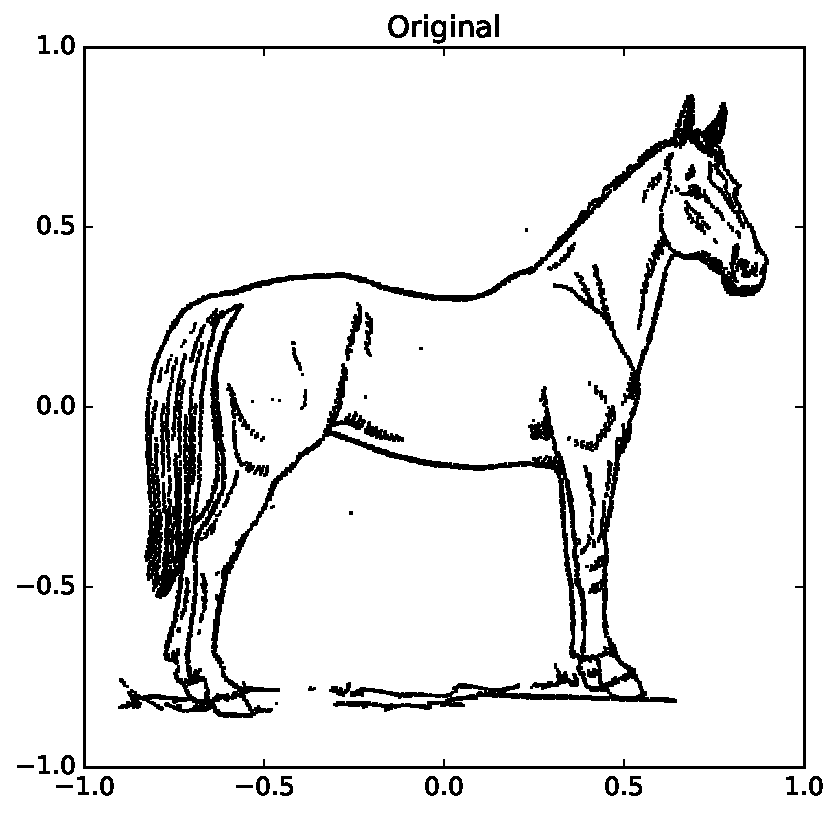
\includegraphics[width=\linewidth]{originalHorse.pdf}
\end{subfigure}%
\begin{subfigure}{.5\textwidth}
    \centering
    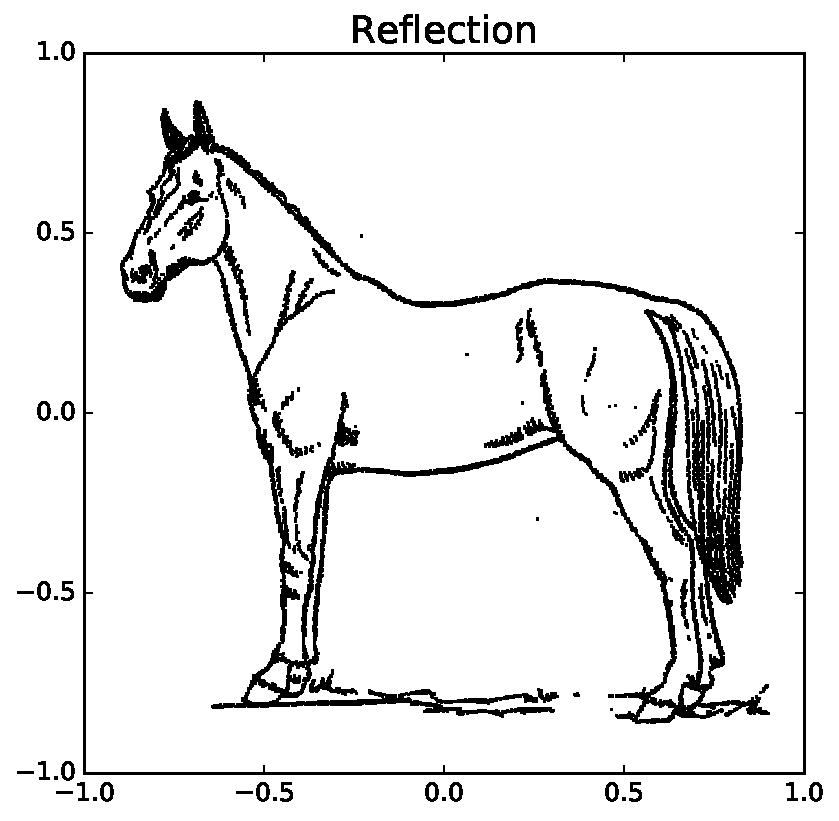
\includegraphics[width=\linewidth]{ReflectionHorse.pdf}
\end{subfigure}
\label{fig:reflect}
\end{figure}

\begin{problem}
Write a function that accepts an array of points and a 1-D array describing the axis of reflection (in the notation above, this argument is $(l_1, l_2)$.
Your function should return the reflected points.
\end{problem}

\subsection*{Composition of linear transformations}
Recall that composition of linear transformations corresponds to matrix multiplication.
For example, if $S$ is a matrix representing a shear and $R$ is a matrix representing a rotation, then $RS$ represents a shear followed by a rotation.

In fact, any linear transformation of $\mathbb{R}^2$ is a composition of the transformations discussed in this lab.
This is because reflections, dilations, and shears provide us with all the elementary matrices, and every matrix is a product of elementary matrices.

% ComboHorse might not be necessary!!

\section*{Affine transformations}
\subsection*{Translations}

A translation is a map $T: \mathbb{R}^2 \rightarrow \mathbb{R}^2$ defined by $T(\mathbf{x}) = \mathbf{x}+\mathbf{b}$ where $\mathbf{b} \in \mathbb{R}^2$.
For example, if $\mathbf{b} = (2, 0)\trp$, then applying $T$ to an image will shift it right by 2.
This translation is illustrated below.

\begin{figure}[H] % Generated with translated_horse() in plots.py.
\captionsetup[subfigure]{justification=centering}
\centering
\begin{subfigure}{.5\textwidth}
    \centering
    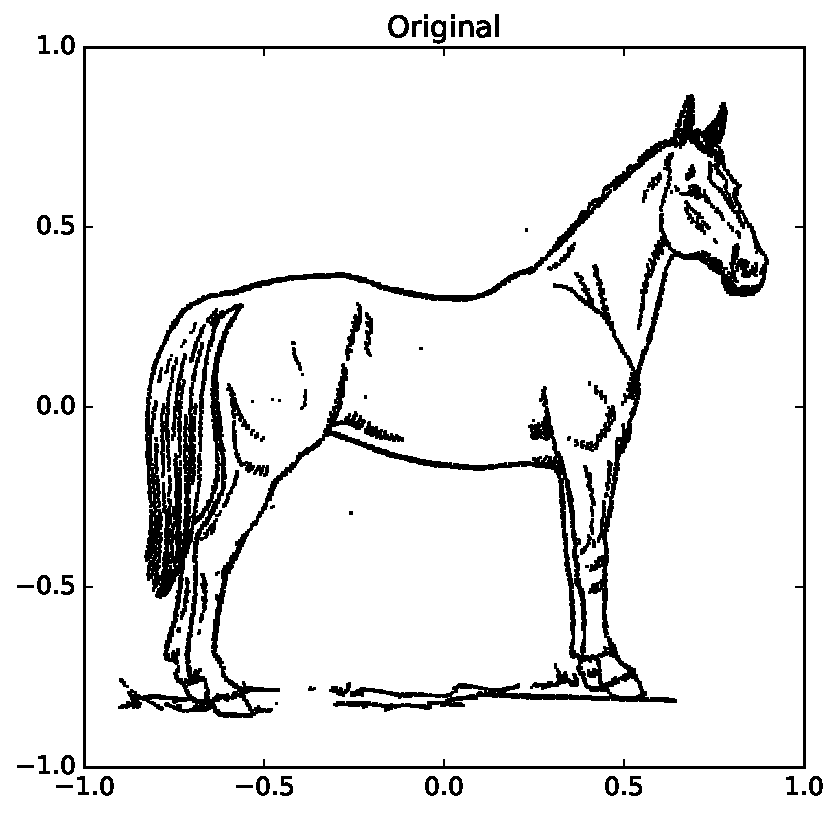
\includegraphics[width=\linewidth]{originalHorse.pdf}
\end{subfigure}%
\begin{subfigure}{.5\textwidth}
    \centering
    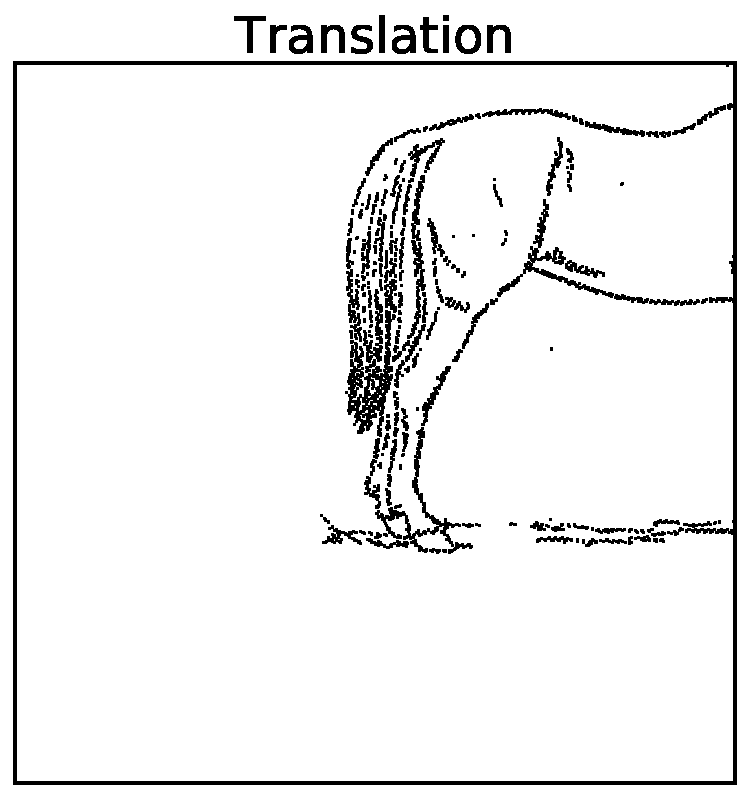
\includegraphics[width=\linewidth]{TranslationHorse.pdf}
\end{subfigure}
\end{figure}

Translations are usually \textbf{not} linear maps.
Therefore, they cannot be represented with matrix multiplication.

\begin{problem}
Write a function that accepts an array of points and an array indicating how much to shift them in each direction.
The function should return the translated points.
Hint: You can construct a $2 \times 1$ array using the syntax \li{np.array([[a], [b]])}.
This may be more convenient for broadcasting.
Another hint: To check your work, plot the original points and their images under the transformation using the function \li{plotOldNew()} defined in Problem \ref{prob:dilation}.
\end{problem}

\subsection*{Affine transformations}
Translations, together, with linear transformations, make up the broader class of transformations called ``affine transformations."
These are transformations of the form $T: \mathbb{R}^2 \to \mathbb{R}^2$, $T(X) = AX + b$ where $A$ is an $n\times n$ matrix and $b \in \mathbb{R}^n$.
Affine transformations include all compositions of scalings, rotations, dilations, reflections, and translations.
For example, if $S$ represents a shear and $R$ a rotation, and if $\mathbf{b}$ is a vector in $\mathbb{R}^2$, then $T(\mathbf{x}) = RS\mathbf{x} + \mathbf{b}$ first shears $\mathbf{x}$, then rotates it, and finally translates it by $\mathbf{b}$.

\begin{problem}
Imagine a particle $p_1$ rotating around a second particle $p_2$ which is moving through $\mathbb{R}^2$ in a straight line.
Suppose $p_2$ begins at the origin and $p_1$ begins at $(1, 0)$.
We can compute the trajectory of $p_1$ using affine transformations.

\begin{enumerate}\label{prob:trajectory}
\item Write a function that returns the position of $p_1$ at a time $t$.
Your function should accept a time $t$, an angular velocity $\omega$, a direction vector $\mathbf{v}$, and a speed $s$.
Assume $p_1$ rotates with angular velocity $\omega$ and $p_2$ moves in the direction of $\mathbf{v}$ with speed $s$.
The location of $p_1$ at time $t$ can be computed as follows:
\begin{itemize}
\item Calculate the position of $p_2$ at time $t$ with the formula $(st/\|\mathbf{v}\|) \mathbf{v}$.
\item Calculate the position of $p_1$ as follows:
\begin{itemize}
\item Rotate $p_1$ by $t\omega$ radians.
\item Translate the resulting vector by the vector equal to the position of $p_2$ at time $t$.
\end{itemize}
\end{itemize}
\end{enumerate}
\item Plot the trajectory of $p_1$ on the time interval $(0, 10)$ assuming $\omega=\pi$, $v=(1, 1)$, and $s=3$.
Your graph should look something like Figure \ref{fig:trajectory}.
\begin{figure}[H]
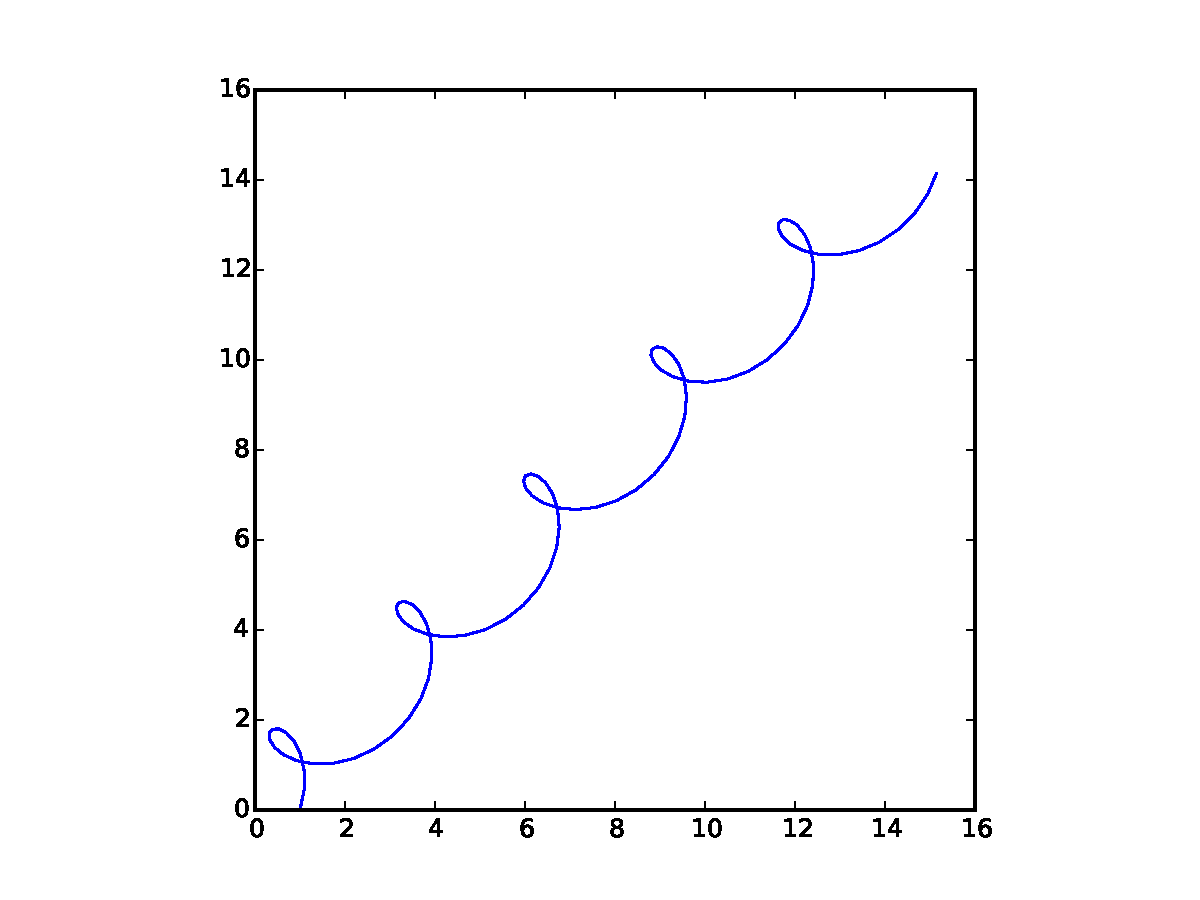
\includegraphics[width=\textwidth]{trajectory.pdf}
\caption{Solution to Problem \ref{prob:trajectory}.}
\label{fig:trajectory}
\end{figure}
\end{problem}
